\section{Demonstration}
% Organize this section according to major topics
% give each topic a section heading in boldface.
% try to cover the major common points :
%
% problem design
% methods of measurement
% supporting models
% supporting data
% simulations run
% results

% Just write the section headings for each part and indicate what goes in that
% section with words :
%
% heading
% figures (with captions)
% schematics (with captions and footnotes)
% equations
% tables

% What does it mean?
% What did I actually test?
% What were the results?
% Did the work yield a new method?
% Did the work yield new knowledge?
% What measurements did I make?
% How were these measurements characterized?
% What methods were used?
% What were the results?
% How were the measurements made and characterized?


The success of the \Cyclus simulator is illustrated by demonstrations
of its fundamental simulation capabilities and the feasibility of \Cyclus
as a community-driven development model.
%The most compelling are demonstrations of the feasibility of the \Cyclus community-driven development 
%model and of fundamental simulation capability. 
Nascent promising growth of the \Cyclus 
The success of the \Cyclus simulator can be measured in many ways. 
The most compelling are demonstrations of the feasibility of the \Cyclus community-driven development 
model and of fundamental simulation capability. Nascent promising growth of the \Cyclus 
ecosystem at multiple institutions indicates that a fuel cycle simulator can 
advance in a community-drive development paradigm. Additionally, simple 
simulations as well as more complex recycling simulations demonstrate that 
\Cyclus possesses fundamental fuel cycle simulation capabilities.

\subsection{Ecosystem}
% Cycamore library
% Cyder?

The \Cyclus `Ecosystem' is the collection of tools, calculation libraries, 
archetypes, data, and input files intended for use with the \Cyclus simulator. 
Members of the ecosystem include:
\begin{itemize}
\item the archetypes provided in the \Cycamore \cite{carlsen_cycamore_2014} 
repository
\item the archetypes created by researchers
\item isotopic composition data
\item historical facility deployment data
\item the \Cyclus \gls{GUI} tool Cyclist
\item fundamental analysis tools in the \Cyclus toolkit
\item tools for \Cyclus optimization, parallelization, and development
\end{itemize}
Taken together, these form an `ecosystem' of capabilities. Over time, this 
ecosystem will grow as archetype-developers, kernel-developers, and 
even users contribute capabilities developed for their own needs. Indeed, the 
long-term vision for the \Cyclus framework predicts an ever-expanding ecosystem 
of both general and specialized capability extensions within the ecosystem. 

Already, the ecosystem is growing. Early cross-institutional contributions to 
the ecosystem demonstrate a significant achievement by the \Cyclus framework 
and provide hope for a community-driven development model. 

\subsubsection{Supplementary Projects}

A number of projects and tools outside of the core simulation kernel have been 
developed which improve the scope and the diversity of the capabilities in the \Cyclus 
ecosystem. Table \ref{tab:coretools} lists the tools and projects developed 
under close integration with the \Cyclus kernel.  These tools are used to ease development
and simulation design (Cystub, Cycic, Ciclus), data visualization and analysis (Cyclist, Cyan),
and remote execution (Cloudlus).

\begin{table}[h]
\centering
\begin{tabularx}{\textwidth}{|r|X|r|}
\hline
\textbf{Name} & \textbf{Description} & \textbf{Citation} \\
\hline
Cycic &  Input control - embedded in Cyclist & \cite{flanagan_input_2013}\\
Cyclist & Interactive data exploration environment & \cite{livnat_cyclist_2014} \\
Ciclus & Continuous integration scripts for \Cyclus & \cite{scopatz_ciclus_2014}\\
Cycstub & Skeleton for clean slate module development & \cite{carlsen_cycstub_2014}\\
Cyan & \Cyclus analysis tool & \cite{carlsen_cyan_2014}\\
Cloudlus & Tools for running \Cyclus in a cloud environment & \cite{carlsen_cloudlus_2014} \\
\hline
\end{tabularx}
\caption{Many tools have been developed outside of the scope of the \Cyclus kernel for improved user, developer, and analyst experiences with \Cyclus.}
\label{tab:coretools}
\end{table}

\subsubsection{Archetype Contributions}

Many archetypes external to the \Cycamore library (Table \table{tab:cycamore})  
have been 
\cite{huff_streamblender_2014,huff_commodconverter_2014}
or are being 
\cite{flanagan_bright-lite_2014,skutnik_nuclear_2014,huff_mktdriveninst_2014} developed for contribution to the 
\Cyclus ecosystem. These archetypes provide the first examples of 
developer-contributed capabilities.  They add to the fundamental \Cycamore
archetypes by providing physics-based reactors, separation, fabrication, and storage
facilities, and expanded institutional paradigms.  These contributed archetypes
illustrate the power of a community-based development approach.

\begin{table}[h]
\centering
\begin{tabularx}{\textwidth}{|r|X|r|}
\hline
\textbf{Name} & \textbf{Description} & \textbf{Citation} \\
\hline
Bright-lite & A physics-based reactor archetype and fuel fabrication archetype & \cite{flanagan_bright-lite_2014} \\
Nuclear Fuel Inventory Model & A flexible, ORIGEN-based, reactor analysis module & \cite{skutnik_nuclear_2014} \\
CommodConverter & A simple commodity converting storage facility archetype  & \cite{huff_commodconverter_2014} \\
MktDrivenInst & An institution that controls deployment based on commodity availability & \cite{huff_mktdriveninst_2014} \\
SeparationsMatrix & A facility for elemental separations of used fuel & \cite{huff_streamblender_2014} \\
StreamBlender & A facility for fuel fabrication from reprocessed streams & \cite{huff_streamblender_2014} \\
\hline
\end{tabularx}
\caption{A diverse set of archetypes under development reflect the diverse 
needs of researchers at various institutions. These archetypes, contributed 
outside of the \Cyclus core and \Cycamore libraries are the first demonstration 
of community-driven development in a fuel cycle simulator.}
\label{tab:archetypes}
\end{table}


\subsection{Simulations}
%Inpro example (is this still running or did we deprecate it with 1.0?)

% MJG - INPRO should be tried again. @rwcarlsen has been running lots of
% simulations with the batch reactor, and its the second generation of my
% reactor models. We could easily use the same demand schedule and enrichment
% facility parameters and run it again.

Results of some simple recycle scenarios run in \Cyclus follow. Beginning with a single
reactor simulation, open (no recycle), modified open, and closed (infinite-pass recycle) 
fuel cycles are compared to illustrate the resolution possible with \Cyclus.  The simulation
is then expanded to include multiple reactors in the same set of fuel cycles to demonstrate
the system-scale convergance to continuous material flow models. 

Because material is tracked as discrete objects, single-pass \gls{MOX} 
recycle is easy to implement in \Cyclus.  The MOX simulation includes one provider of fresh
\gls{UOX} fuel, one recycled fuel fabrication facility, one reactor, one separations
facility, and one repository. The simulation has a duration of 1100 months and a \TODO{??-month stepsize}.

%** full-system plutonium buildup for open
(no recycle), modified open, and closed (infinite-pass recycle) variations of
%the scenario described above (all just a single reactor).  **

The \Class{BatchReactor} archetype from \Cycamore has the ability to accept
fuel materials from an arbitrary number of different sources, delineated by
commodity. Custom, non-uniform preferences can be set for each different fuel
commodity.  The dynamic resource exchange makes it easy for a reactor to
preferentially accept recycled \gls{MOX} fuel over fresh \gls{UOX} fuel.  In this
simulation, the
\Class{BatchReactor} was configured to run with a 3 batch core on 18 month cycles and
a 2-month refueling period.  Adjusting and setting parameters such as these is
as simple as editing numbers in an input file such as:

\begin{lstlisting}[language=xml]
  ...
  <BatchReactor>
      ...
      <processtime>18</processtime>
      <nbatches>3</nbatches>
      <batchsize>20000</batchsize>
      <refueltime>2</refueltime>
      ...
  </BatchReactor>
  ...
\end{lstlisting}

The \Class{Source} and \Class{Sink} archetypes from \Cycamore have been used as a
source of fresh, enriched uranium and a repository respectively. A simple
custom recycled fuel fabrication facility was also used, which mixes fissile 
and fertile streams to match target fuel compositions as closely
as possible.  The method used for this matching is approximately the same as
that used by the \gls{COSI} fuel cycle simulator \TODO{cite COSI equivalence
method}. The material flows for this simulation are shown below in figure
\ref{fig:flowmodopen}.

\begin{figure}[H]
\label{fig:flowmodopen}
\caption{Modified open 1-pass \gls{MOX} recycle fuel cycle material flows.}
\begin{center}
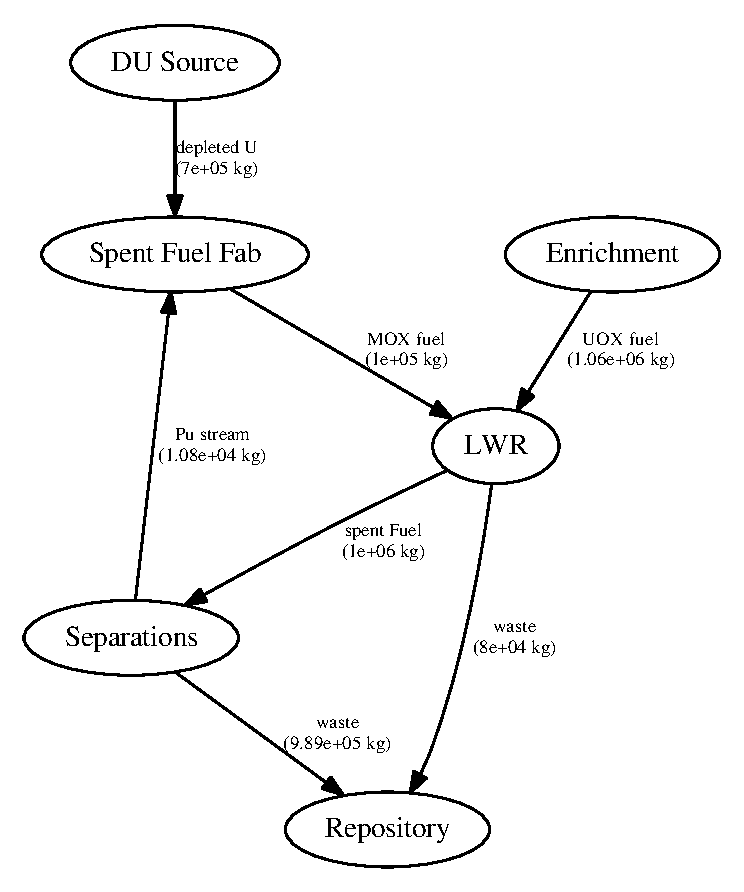
\includegraphics{./images/flow-mod-open-1.eps}
\end{center}
\end{figure}

To switch to a fully closed fuel cycle, all that needs to be done is change
the output commodity for the spent \gls{MOX} fuel of the \Class{BatchReactor}, 
requiring only a one-word change in the input file: 

\begin{lstlisting}[language=diff]
  --- mod-open-1.xml	2014-10-08 08:31:33.892523173 -0500
  +++ closed-1.xml	2014-10-08 08:31:33.892523173 -0500
  @@ -108,7 +108,7 @@
           <fuel>         
             <incommodity>mox_fuel</incommodity>
             <inrecipe>lwr_mox_fuel</inrecipe>
  -          <outcommodity>spent_mox</outcommodity>
  +          <outcommodity>spent_fuel</outcommodity>
             <outrecipe>mox_spent_fuel</outrecipe>
           </fuel>
\end{lstlisting}

This results in new the material flows in Figure \ref{fig:flowclosed}. Note
that because the \Class{BatchReactor} always transmutes fuel into the same
composition, the nuclide level flows are not very realistic for the full, 
multi-pass
recycle case.

\begin{figure}[H]
\label{fig:flowclosed}
\caption{Full \gls{MOX} recycle (multi-pass) fuel cycle material flows.}
\begin{center}
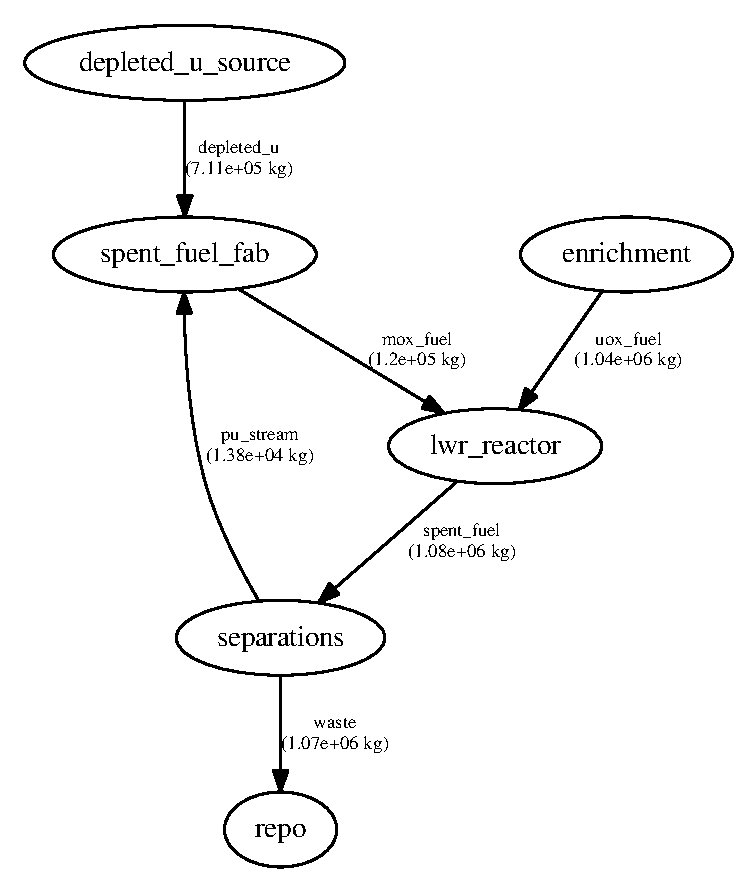
\includegraphics{./images/flow-closed-1.eps}
\end{center}
\end{figure}

Figure \ref{fig:puseries1} shows the full-system plutonium buildup for open
(no recycle), modified open, and closed (infinite-pass recycle) variations of
the scenario described above (all just a single reactor).  The figure was
generated directly from \Cyclus output data. After several batch cycles (near
month 300) in the modified open and closed cases, enough separated fissile
material accumulates in the fuel fabrication facility to generate a full
recycled batch.  When this batch is transmuted, more plutonium is burned than
created.  This results in a drop in the total fuel cycle system plutonium
inventory.  This pattern repeats roughly every 10 cycles (200 months) for the
modified open case and every 9 cycles (180 months) for the closed case.
Because the modified open scenario does not re-recycle material, it takes the
fabrication facility 1 cycle longer to accumulate a full batch worth of
fissile material. 

Because facilities are represented individually and
transact discrete materials as discrete events, realistic non-uniform patterns in facility behavior
that affect total system behavior are observed using \Cyclus, which is uncommon 
for fleet-based, continuous material flow models.

\begin{figure}[H]
\label{fig:puseries1}
\caption{System plutonium buildup with one reactor.}
\begin{center}
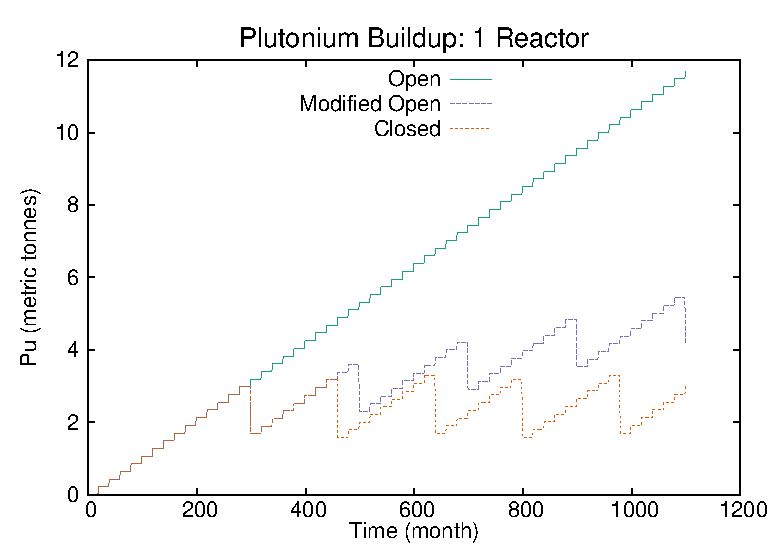
\includegraphics{./images/puseries-1.eps}
\end{center}
\end{figure}

The open, modified open, and closed scenarios can easily be modified to have
several reactors each with staggered refueling times. The plutonium buildup
for these three multi-reactor variations is shown in Figure
\ref{fig:puseriesn}. As the number of
reactors increases, the behavior of the system approaches a more steady
average reminiscent of continuous material flow models. 

\begin{figure}[H]
\label{fig:puseriesn}
\caption{System plutonium buildup with staggered refueling for many reactors.}
\begin{center}
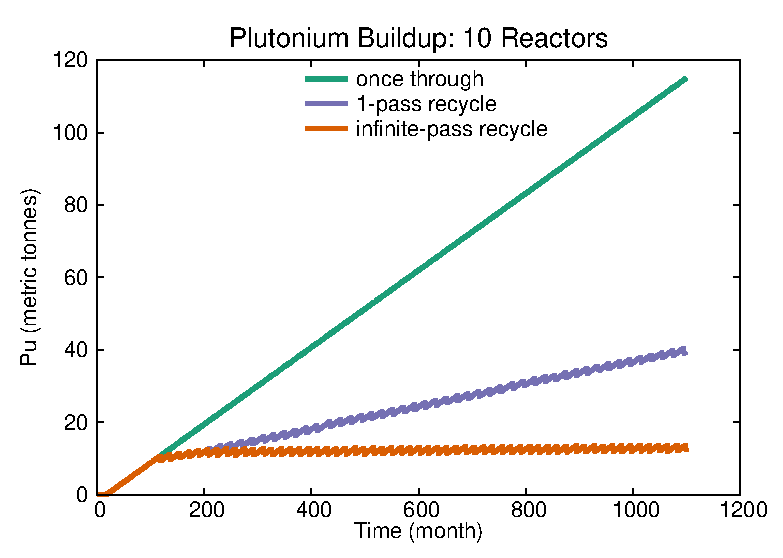
\includegraphics{./images/puseries-n.eps}
\end{center}
\end{figure}

